\section{Each format against JSON, by regime}
\label{sec:against-json}

The tables of this appendix give every format against JSON on the same case,
as a geometric mean over the cases the format carries, with the web and bulk
regimes apart; below 1 is smaller or faster than JSON. Because formats
differ in the cases they carry, two formats' means here are not directly
comparable; Section~\ref{sec:results} compares \colbin{} with each format on
the cases both carry. Tables~\ref{tab:versus-web} and~\ref{tab:versus-bulk}
do the same by regime, with \colbin{}'s own variants.

\begin{table}[ht]
\centering\small
\resulttable{sizes-web}
\caption{Web regime: message size against JSON's, as written (\emph{raw})
and under each compressor, both sides compressed alike. $\dagger$: cases
where the format writes zero bytes are left out of the mean.}
\label{tab:sizes-web}
\end{table}

\begin{table}[ht]
\centering\small
\resulttable{sizes-bulk}
\caption{Bulk regime: message size against JSON's.}
\label{tab:sizes-bulk}
\end{table}

\begin{table}[ht]
\centering\footnotesize
\resulttable{sizes-datasets-web}
\caption{Web regime by dataset: size against JSON's, as written and under
gzip.}
\label{tab:sizes-datasets-web}
\end{table}

\begin{table}[ht]
\centering\small
\resulttable{times-web}
\caption{Web regime: time against JSON's for the same operation
(\result{time.web.cases} cases; access against JSON's decode-fresh, on the
\result{time.web.access.cases} cases that have an access aggregate).}
\label{tab:times-web}
\end{table}

\begin{table}[ht]
\centering\small
\resulttable{times-bulk}
\caption{Bulk regime: time against JSON's for the same operation
(\result{time.bulk.cases} cases).}
\label{tab:times-bulk}
\end{table}

\begin{table}[ht]
\centering\footnotesize
\resulttable{versus-web}
\caption{Web regime: \colbin{}'s number over each other format's, as a
geometric mean over the cases both carry, and in small type the number of
those cases in which \colbin{}'s is strictly lower. Below 1, \colbin{} is
smaller or faster.}
\label{tab:versus-web}
\end{table}

\begin{table}[ht]
\centering\footnotesize
\resulttable{versus-bulk}
\caption{Bulk regime: \colbin{} against each other format on common cases.}
\label{tab:versus-bulk}
\end{table}

\begin{figure}[ht]
\centering
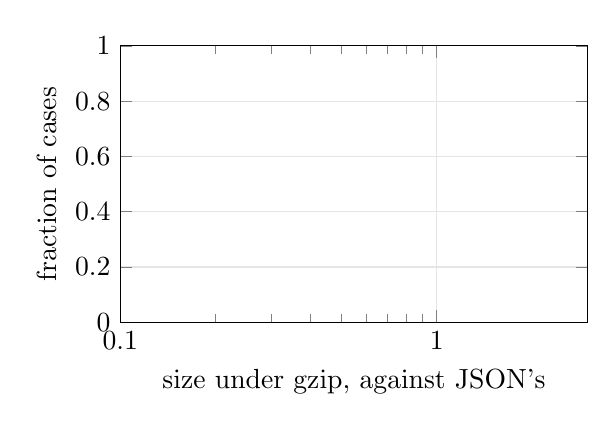
\begin{tikzpicture}
\begin{axis}[width=0.62\linewidth, height=0.42\linewidth,
  xlabel={size under gzip, against JSON's}, ylabel={fraction of cases},
  xmode=log, log ticks with fixed point, xmin=0.1, xmax=3, ymin=0, ymax=1,
  legend pos=outer north east, legend style={font=\footnotesize, draw=none},
  cycle list name=color list, grid=major, grid style={gray!20}]
\distcurve{very thick, black}{fig-dist-web-gzip-colbin}{colbin}
\distcurve{thick, blue}{fig-dist-web-gzip-protobuf}{protobuf}
\distcurve{thick, red}{fig-dist-web-gzip-avro}{avro}
\distcurve{thick, orange}{fig-dist-web-gzip-msgpack}{msgpack}
\distcurve{thick, teal}{fig-dist-web-gzip-arrow}{arrow}
\distcurve{thick, gray}{fig-dist-web-gzip-flatbuffers}{flatbuffers}
\end{axis}
\end{tikzpicture}
\caption{Web regime: the distribution over cases of each format's size under
gzip against JSON's under gzip. A curve to the left is smaller; each
format's curve is over the cases it carries.}
\label{fig:dist-size}
\end{figure}

\begin{figure}[ht]
\centering
\begin{tikzpicture}
\begin{axis}[width=0.48\linewidth, height=0.44\linewidth, title={web},
  xlabel={size under gzip}, ylabel={decode-fresh time},
  xmode=log, ymode=log, log ticks with fixed point,
  nodes near coords, point meta=explicit symbolic,
  every node near coord/.append style={font=\tiny, anchor=west},
  grid=major, grid style={gray!20}, enlarge x limits=0.25]
\IfFileExists{\tables/fig-tradeoff-web.dat}{
  \addplot[only marks, mark=*, mark size=1.5pt] table[x=gzip, y=decode, meta=format]{\tables/fig-tradeoff-web.dat};}{}
\end{axis}
\end{tikzpicture}\hfill
\begin{tikzpicture}
\begin{axis}[width=0.48\linewidth, height=0.44\linewidth, title={bulk},
  xlabel={size under gzip},
  xmode=log, ymode=log, log ticks with fixed point,
  nodes near coords, point meta=explicit symbolic,
  every node near coord/.append style={font=\tiny, anchor=west},
  grid=major, grid style={gray!20}, enlarge x limits=0.25]
\IfFileExists{\tables/fig-tradeoff-bulk.dat}{
  \addplot[only marks, mark=*, mark size=1.5pt] table[x=gzip, y=decode, meta=format]{\tables/fig-tradeoff-bulk.dat};}{}
\end{axis}
\end{tikzpicture}
\caption{Size against decode time, both against JSON's, per format and
regime (geometric means; each format over the cases it carries). Down and to
the left is better on both.}
\label{fig:tradeoff}
\end{figure}
